\chapter{Задание \textnumero2}

\section{Условие}
Написать приложение по модели клиент-сервер, осуществляющее взаимодействие параллельных процессов, которые выполняются на разных компьютерах. Для взаимодействия с клиентами сервер должен использовать мультиплексирование. Сервер должен обслуживать запросы параллельно запущенных клиентов. При демонстрации работы программного комплекса необходимо запустить несколько клиентов (не меньше 5) и продемонстрировать, что сервер обрабатывает обращения каждого запущенного клиента.

\section{Реализация}

\sloppy В процессе-сервере при помощи системного вызова socket создается сетевой сокет семейства AF\_INET и типа SOCK\_STREAM\@. Системный вызов bind связывает сокет с адресом. Далее процесс-сервер при помощи listen переводится в режим ожидания запроса на соединение от процессов-клиентов. После этого процесс-сервер блокируется системным вызовом select, который возвращает управление при поступлении запроса от процесса-клиента. В этом случае процесс-сервер производит проверку на появление нового соединения от процесса-клиента и при его наличии вызывает функцию \_connect. В этой функции устанавливается новое соединение при помощи вызова функции accept и создается еще один сокет, который затем заносится в массив файловых дескрипторов. После этого происходит вызов функции \_serve\_clients, в которой производится обход массива файловых дескрипторов и проверка, находится ли конкретный файловый дескриптор в наборе дескрипторов (проверка производится при помощи макроса FD\_ISSET). Если находится, то при помощи функции read процессом-сервером считывается сообщение от процесса-клиента. Если вызов read вернул нулевое значение, то сокет закрывается и удаляется из массива файловых дескрипторов. Иначе выводится полученное сообщение. Текст программы-сервера приведён в листинге~\ref{lst:netserver}.

\begin{lstlisting}[caption={Текст программы-сервера},label=lst:netserver]
#include <stdio.h>
#include <errno.h>
#include <unistd.h>
#include <signal.h>
#include <stdlib.h>
#include <string.h>
#include <sys/types.h>
#include <sys/socket.h>
#include <sys/select.h>
#include <netinet/in.h>

#define LISTENQTY 256
#define FEEDBACK_MSG "Ok"

static int socket_fd;
static int greatest_fd;
static int greatest_idx;

static void show_usage(char  *pname);
static void handle_sigint(int signum);

static int _connect(int *client_fds, int *client_pids,
                    fd_set *fdset);
static int _serve_clients(int *client_fds, int *client_pids,
                          fd_set *fdset, fd_set *reset);

int main(int argc, char **argv)
{
    int port;
    struct sockaddr_in server_addr;

    signal(SIGINT, &handle_sigint);

    if (argc < 2)
    {
        show_usage(argv[0]);
        exit(1);
    }
    else
    {
        char *endptr;

        port = strtol(argv[1], &endptr, 10);

        if (*argv[1] == 0 || *endptr != 0)
        {
            show_usage(argv[0]);
            exit(1);
        }
    }

    greatest_fd = socket_fd = socket(AF_INET, SOCK_STREAM, 0);

    if (socket_fd < 0)
    {
        fprintf(stderr, "%s: %s\n", "socket", strerror(errno));
        exit(1);
    }

    memset(&server_addr, 0, sizeof(server_addr));

    server_addr.sin_family = AF_INET;
    server_addr.sin_addr.s_addr = INADDR_ANY;
    server_addr.sin_port = htons(port);

    if (bind(socket_fd,
             (struct sockaddr *)&server_addr,
             sizeof(server_addr)) < 0)
    {
        fprintf(stderr, "%s: %s\n", "bind", strerror(errno));
        exit(1);
    }

    listen(socket_fd, LISTENQTY);

    int client_fds[FD_SETSIZE];
    int client_pids[FD_SETSIZE];
    fd_set fdset;
    fd_set reset;

    for (int i = 0; i < FD_SETSIZE; ++i)
        client_fds[i] = -1;

    FD_ZERO(&fdset);
    FD_SET(socket_fd, &fdset);

    for (;;)
    {
        reset = fdset;
        select(greatest_fd + 1, &reset, NULL, NULL, NULL);

        if (FD_ISSET(socket_fd, &reset))
            if (_connect(client_fds, client_pids, &fdset) != 0)
                {
                    fprintf(stderr, "%s: %s\n",
                            "_connect", strerror(errno));
                    exit(1);
                }

        if (_serve_clients(client_fds, client_pids, &fdset, &reset) != 0)
        {
            fprintf(stderr, "%s: %s\n", "_serve_clients", strerror(errno));
            exit(1);
        }
    }
}

static int _connect(int *client_fds, int *client_pids, fd_set *fdset)
{
    int idx;
    int accepted_fd;
    char buf[BUFSIZ] = { 0 };

    accepted_fd = accept(socket_fd, NULL, NULL);

    if (accepted_fd < 0)
        return 1;

    for (idx = 0; idx < FD_SETSIZE && client_fds[idx] >= 0; ++idx);
    if (idx == FD_SETSIZE)
    {
        errno = ENOMEM;
        return 1;
    }

    FD_SET(accepted_fd, fdset);
    client_fds[idx] = accepted_fd;

    if (greatest_fd < accepted_fd)
        greatest_fd = accepted_fd;
    if (greatest_idx < idx)
        greatest_idx = idx;

    client_pids += idx;
    idx = read(accepted_fd, buf, sizeof(buf) - 1);
    *client_pids = atoi(buf);

    printf("Client (pid %d) just connected\n", *client_pids);

    return 0;
}

static int _serve_clients(int *client_fds, int *client_pids,
                          fd_set *fdset, fd_set *reset)
{
    int read_cnt;
    char buf[BUFSIZ] = { 0 };

    for (int i = 0; i <= greatest_idx; ++i)
        if (FD_ISSET(client_fds[i], reset))
        {
            read_cnt = read(client_fds[i], buf, sizeof(buf) - 1);

            if (read_cnt > 0)
            {
                write(client_fds[i], FEEDBACK_MSG, strlen(FEEDBACK_MSG));

                buf[read_cnt] = '\0';
                printf("Client (pid %d): %s", client_pids[i], buf);
            }
            else
            {
                FD_CLR(client_fds[i], fdset);
                close(client_fds[i]);
                client_fds[i] = -1;
                printf("Client (pid %d) just disconnected\n",
                       client_pids[i]);
            }
        }

    return 0;
}

static void show_usage(char *pname)
{
    fprintf(stderr, "Usage:\n\t%s <port-number>\n", pname);
}

static void handle_sigint(int signum)
{
    close(socket_fd);

    exit(0);
}
\end{lstlisting}

Программа-клиент создает сокет с такими же параметрами, как и программа-сервер. Далее вызывается функция connect, которая устанавливает соединение с сокетом процесса-сервера. При помощи системного вызова write производится отправка сообщений сообщений процессу-серверу, а при помощи read~--- получение. Текст программы-клиента приведён в листинге~\ref{lst:netclient}.

\begin{lstlisting}[caption={Текст программы-клиента},label=lst:netclient]
#include <stdio.h>
#include <errno.h>
#include <netdb.h>
#include <unistd.h>
#include <signal.h>
#include <stdlib.h>
#include <string.h>
#include <sys/types.h>
#include <sys/socket.h>
#include <sys/select.h>
#include <netinet/in.h>

static void show_usage(char  *pname);
static int get_input(char *buf, size_t bufsize);

int main(int argc, char **argv)
{
    int port;
    int socket_fd;
    struct hostent *host;
    struct sockaddr_in server_addr;

    if (argc < 3)
    {
        show_usage(argv[0]);
        exit(1);
    }
    else
    {
        char *endptr;

        port = strtol(argv[2], &endptr, 10);

        if (*argv[2] == 0 || *endptr != 0)
        {
            show_usage(argv[0]);
            exit(1);
        }

        host = gethostbyname(argv[1]);

        if (!host)
        {
            fprintf(stderr, "%s: %s\n", "gethostbyname", strerror(errno));
            exit(1);
        }
    }

    socket_fd = socket(AF_INET, SOCK_STREAM, 0);

    if (socket_fd < 0)
    {
        fprintf(stderr, "%s: %s\n", "socket", strerror(errno));
        exit(1);
    }

    memset(&server_addr, 0, sizeof(server_addr));

    server_addr.sin_family = AF_INET;
    memcpy(&server_addr.sin_addr, host->h_addr_list[0], host->h_length);
    server_addr.sin_port = htons(port);

    if (connect(socket_fd,
                (struct sockaddr *)&server_addr,
                sizeof(server_addr)) < 0)
    {
        fprintf(stderr, "%s: %s\n", "connect", strerror(errno));
        exit(1);
    }

    int read_cnt;
    char buf[BUFSIZ] = { 0 };

    snprintf(buf, sizeof(buf), "%d", getpid());
    write(socket_fd, buf, strlen(buf));

    while (get_input(buf, sizeof(buf)))
    {
        write(socket_fd, buf, strlen(buf));

        read_cnt = read(socket_fd, buf, sizeof(buf) - 1);
        buf[read_cnt] = '\0';
        printf("feedback: %s\n", buf);
    }

    close(socket_fd);
}

static int get_input(char *buf, size_t bufsize)
{
    printf("> ");
    fgets(buf, bufsize, stdin);

    return !feof(stdin);
}

static void show_usage(char *pname)
{
    fprintf(stderr, "Usage:\n\t%s <host-name> <port-number>\n", pname);
}
\end{lstlisting}

\section{Пример работы}

На рисунке~\ref{img:task02} изображён пример работы реализованных программ.

\begin{figure}[H]
    \centering
    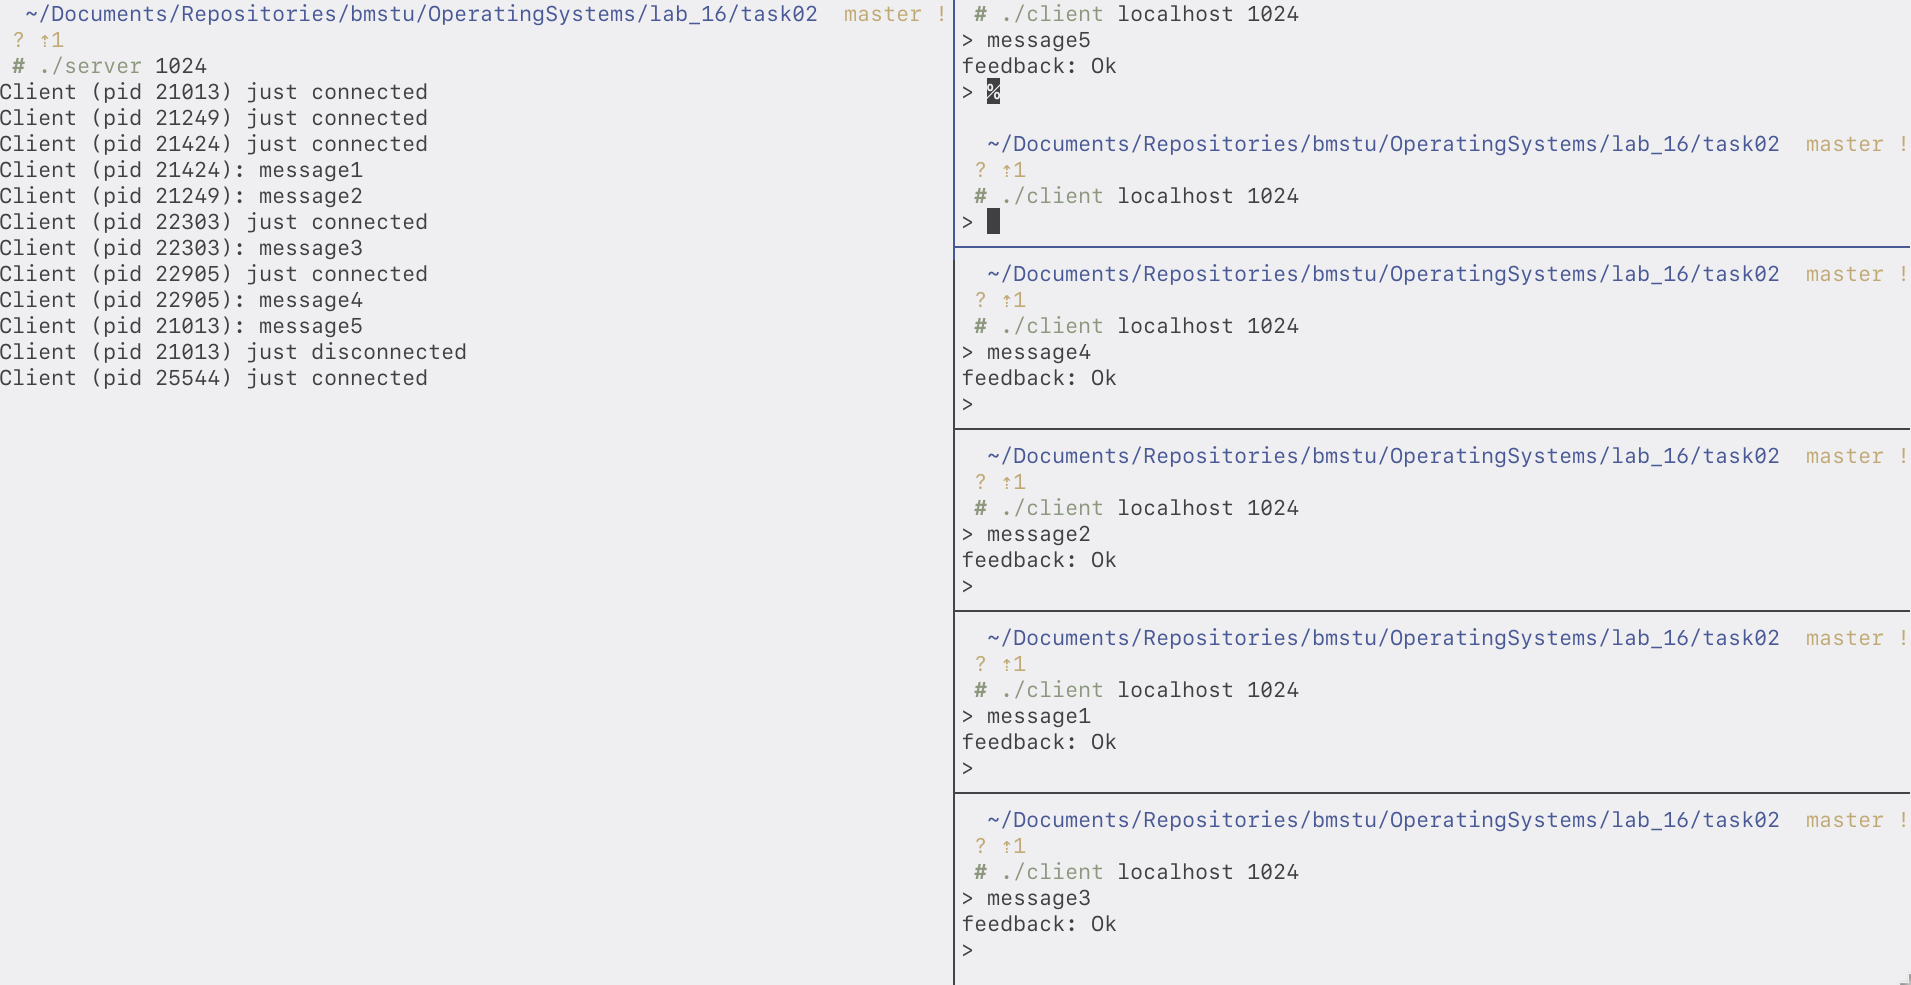
\includegraphics[scale=0.235]{images/task02.png}
    \caption{Задание \textnumero2}\label{img:task02}
\end{figure}

На рисунке~\ref{img:check02} демонстрируется слушающий сокет и связанный с ним порт. Для этого используется команда ss с флагом -l, который включает отображение только слушающих сокетов, и флагом -t, который включает отображение только TCP сокетов.

\begin{figure}[H]
    \centering
    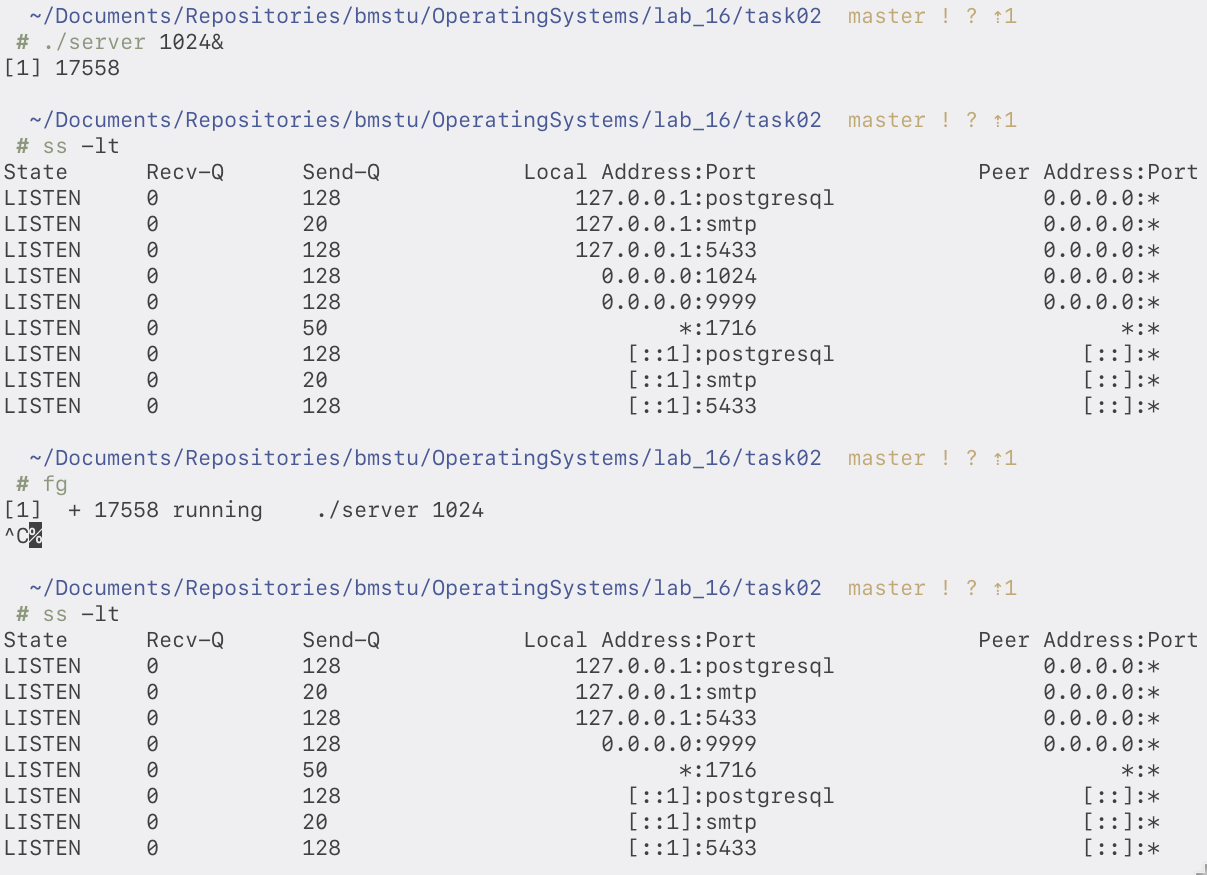
\includegraphics[scale=0.35]{images/check02.png}
    \caption{Демонстрация слушающего сокета}\label{img:check02}
\end{figure}

